% Motivation
    %% Coating Thermal Noise
	%%% Brownian Thermal Noise
	    %%%% Internal Friction in Materials and Loss Angle
    	    %%%% Coating Brownian Thermal Noise
    	    %%%% Silica Ti-Tantala coating parameters
    	    %%%% GaAs/AlGaAs coating parameters
    %% Anisotropic Media
	%%% The Dielectric Tensor
    	%%% Indicatrix
    	%%% Linear Electro-optic Effect (Pockel's Effect)
    	%%% Electro-optic coefficients r_ij for zincblende crystals
    	%%% New Principal (electro-optic) dielectric constants for zincblende structures
    	%%% The photoelastic effect
    	%%% The generalized indicatrix
    %% EO modulation
    %% Optical anisotropy of an HR GaAs / AlGaAs stack
    %% Miller indices for HR GaAs / AlGaAs coatings
        %%% Electro-optic coupling to the reflected phase of a HR mirror coating
    %% Numerical estimate
    %% Measured birefringence from HR \texorpdfstring{$\gaas$}{gaas}/\texorpdfstring{$\algaas$}{algaas} mirrors
    %% Initial projected DARM coupling

\section{Motivation}
Contributions of categorized noises for gravitational wave detectors are organized in a ``noise budget" (i.e. \autoref{fig:aplusasharp} and \autoref{fig:high_freqnoise}): comprised of a collection of technical (noise imposed by the practical operation of the detector) and fundamental (inherent physical limitations of the DRFPMI design) noise that limit gravitational wave detection. Understanding how much differential phase noise is imparted on the interferometer carrier light passing through and reflecting from core optics is crucial. This section contains targeted discussions of coating thermal noise from highly reflective coatings as well as electro-optic noise from highly reflective crystalline coatings to motivate the construction and measurement of a calibrated estimate of the electro-optic noise from $\gaas$/$\algaas$ coatings.

\subsection{Coating Thermal Noise}
%% Contributions of categorized noises for gravitational wave detectors the ''noise budget" ((LHO and LLO O3?) or just GWINC?)}
One source of noise in high precision optical experiments operating at room temperature (and higher due to high power resonant beams), can be realized through Brownian thermal noise and the Fluctutaion dissapation theorem. 

\subsubsection*{Brownian Noise}
In 1827 the Scottish botanist Robert Brown observed a constant motion of pollen particulates on the surface of water; witnessing randomized collisions of the water molecules holding a kinetic energy proportional to the temperature ($k_BT$) \cite{brown:1828}. It is because of these documented observations we name the phenomena Brownian motion. And although the observations were on motion of particulates in liquids and gases, solids also exhibit similar fluctuations through their modes of dissipation. 

\subsubsection*{Fluctuation Dissipation Theorem}
Any movement or fluctuation in the core optic components at finite temperatures holds particular significance for gravitational wave detectors; this becomes clearer when reviewing the fluctuation dissipation theorem. Derived by H.B. Callen and T.A. Welton, the theorem states that for a randomly fluctuating linear force ($F_x^2(f)$) \cite{callen:1951}:

%% Further insight into Brownian motion was explored by Einstein where he was able to relate the mean-square displacement of a particle of radius $r_\mathrm{sph}$ on a fluid with viscosity $\eta$.
 %%\begin{equation}
 %%\overline{x^2} = k_B T  \frac{1}{3 \pi \eta  r_\mathrm{sph}}
 %%\end{equation}
 %%This relation has important implications about how the random motion or fluctuations of a particulate (the pollen) is influenced (dissipated) by the viscosity of the surrounding medium (water).

\begin{equation}
F_x^2(f) = 4 k_B T\; \Re[Z]
\end{equation}

\noindent Where $\Re[Z]$ is the real part of the impedance of the system. This impedance directly relates to equations of motion:

 \begin{equation}
 Z = \frac{F}{\dot{x}}
 \end{equation}

 \noindent Another useful form is the power spectrum of the fluctuating motion:

\begin{equation}\label{eq:fdtpsd}
x^2 (f)  = \frac{4k_B T}{(2 \pi f)^2}\; \Re[Y]
\end{equation}

\noindent Where $Y$ is the inverse impedance or admittance. The root mean square (RMS) displacement ($x^2(f)$) as informed by the FDT facilitates modelling and budgeting notable Brownian noise sources that fundamentally limit LIGO (i.e. by choice of materials used for highly reflective mirror coatings). Though adequate modelling of internal force couplings for the aforementioned components provides a more complete picture.

\subsubsection*{Internal friction in materials and loss angle}
Zener provides a model of the internal friction of materials incorporating anelasticity into the equations of motion \cite{zener:1948}:
\begin{equation}
F = k(1+i\phi)x + m\ddot{x}
\end{equation}

\noindent Where $m$ is mass attached to a spring with a spring constant $k(1+ i\phi)$ incorporating the degree of anelasticity $\phi$. From equations 3.5 and 3.3 we perform a Laplace transform and acquire the following form of admittance:
\begin{equation}
Y(s) = \frac{\dot{x}(s)}{F(s)} = \frac{-s}{k(1+i\phi) + ms^2}
\end{equation}

\noindent Or more transparently the Fourier representation since we assume a linear time invariant system:

\begin{equation}\label{eq:admitint}
Y(\omega) = \frac{\dot{x}(\omega)}{F(\omega)} = \frac{-i\omega}{k(1+i\phi) - m\omega^2} = \frac{k \omega \phi - i \omega (k - m \omega^2)}{(k-m\omega^2)^2 +k^2 \phi^2}
\end{equation}

\noindent Plugging equation \autoref{eq:admitint} back into \autoref{eq:fdtpsd}:

\begin{equation}
x^2 (f)  = \frac{2k_B T}{\pi}\frac{k\phi}{(k-4\pi^2 m f^2)^2 + k^2 \phi^2}
\end{equation}

Computing the admittance from a Gaussian beam impinging upon a HR mirror can require expansion of all individual mechanical degrees of freedom of the test mass system across a relevant frequency range, and with such an approach convergence is not guaranteed. Saulson and Gonzalez provide an alternative method to computing the admittance coined the ``direct approach" by Levin when computing the noise from a Gaussian beam on a LIGO HR test mass. The admittance can be acquired through:

\begin{equation}\label{eq:admitdirec}
\Re[Y] = \frac{W_\mathrm{diss}}{F_o^2}
\end{equation}

\noindent $W_\mathrm{diss}$ is the dissipated power from the system due to an oscillating force $F_o$. This form of the admittance reveals an important result of the fluctuation dissapation theorem where an undriven system with a dissapative actor, imparts motion to the degrees of freedom via a driving force by virtue of that same actor at finite temperatures. This direct approach also allows the surface pressure applied by the Gaussian beam to interrogate which mechanical modes of the test mass impose a significant energy when \autoref{eq:admitdirec} is plugged into \autoref{eq:fdtpsd}. In the case of the gaussian beam / uncoated test mass studied by Levin \cite{levin:1998}:

\begin{equation}
S_x(f) = \frac{4 k_B T}{f} \frac{1-\sigma^2}{\pi^3 E_o r_o} I\phi \bigg[1- O\bigg( \frac{r_o}{R} \bigg)\bigg]
\end{equation}

%this requires that the driving force used in a lab mimics that of a force from a centered Gaussian beam.

%%Refer to Levin appendix for more on how elasticity parameters are introduced?
\noindent Where $\sigma$ and $E_o$ are the Poisson ratio and Young's modulus respectively, and $O(\frac{r_o}{R})$ is a correction term as a function of the small beam radius ($r_o$) relative to the mirror radius ($R$).

\subsubsection*{Thermal noise of HR mirror coatings}
Further investigations into the beam/optic system utilizing this approach and elasticity theory led to a deeper understanding about Brownian thermal noise contributions from LIGO test masses (substrate, suspensions, HR coating). Levin mentions, with further detail from Harry, that the noise contributed by a lossy mirror coating is proven to be to be the most significant contributor of brownian thermal noise ~\cite{harry:2006}. Hong provides a power spectral density \cite{hong:2013}:

\begin{equation}
S_j^X = \frac{4k_B T \lambda \phi_x^j(1- \sigma_j - 2 \sigma_j^2)}{3 \pi^2 f Y_j (1-\sigma_j)^2 \omega_o^2}
\end{equation}
/
\noindent Where X represents bulk and shear with j = odd (material 1) and j = even (material 2) alternating layers representing high and low index materials j = odd (material 1) j = even (material 2) for an HR coating.

\begin{figure}[H]
    \begin{center}
    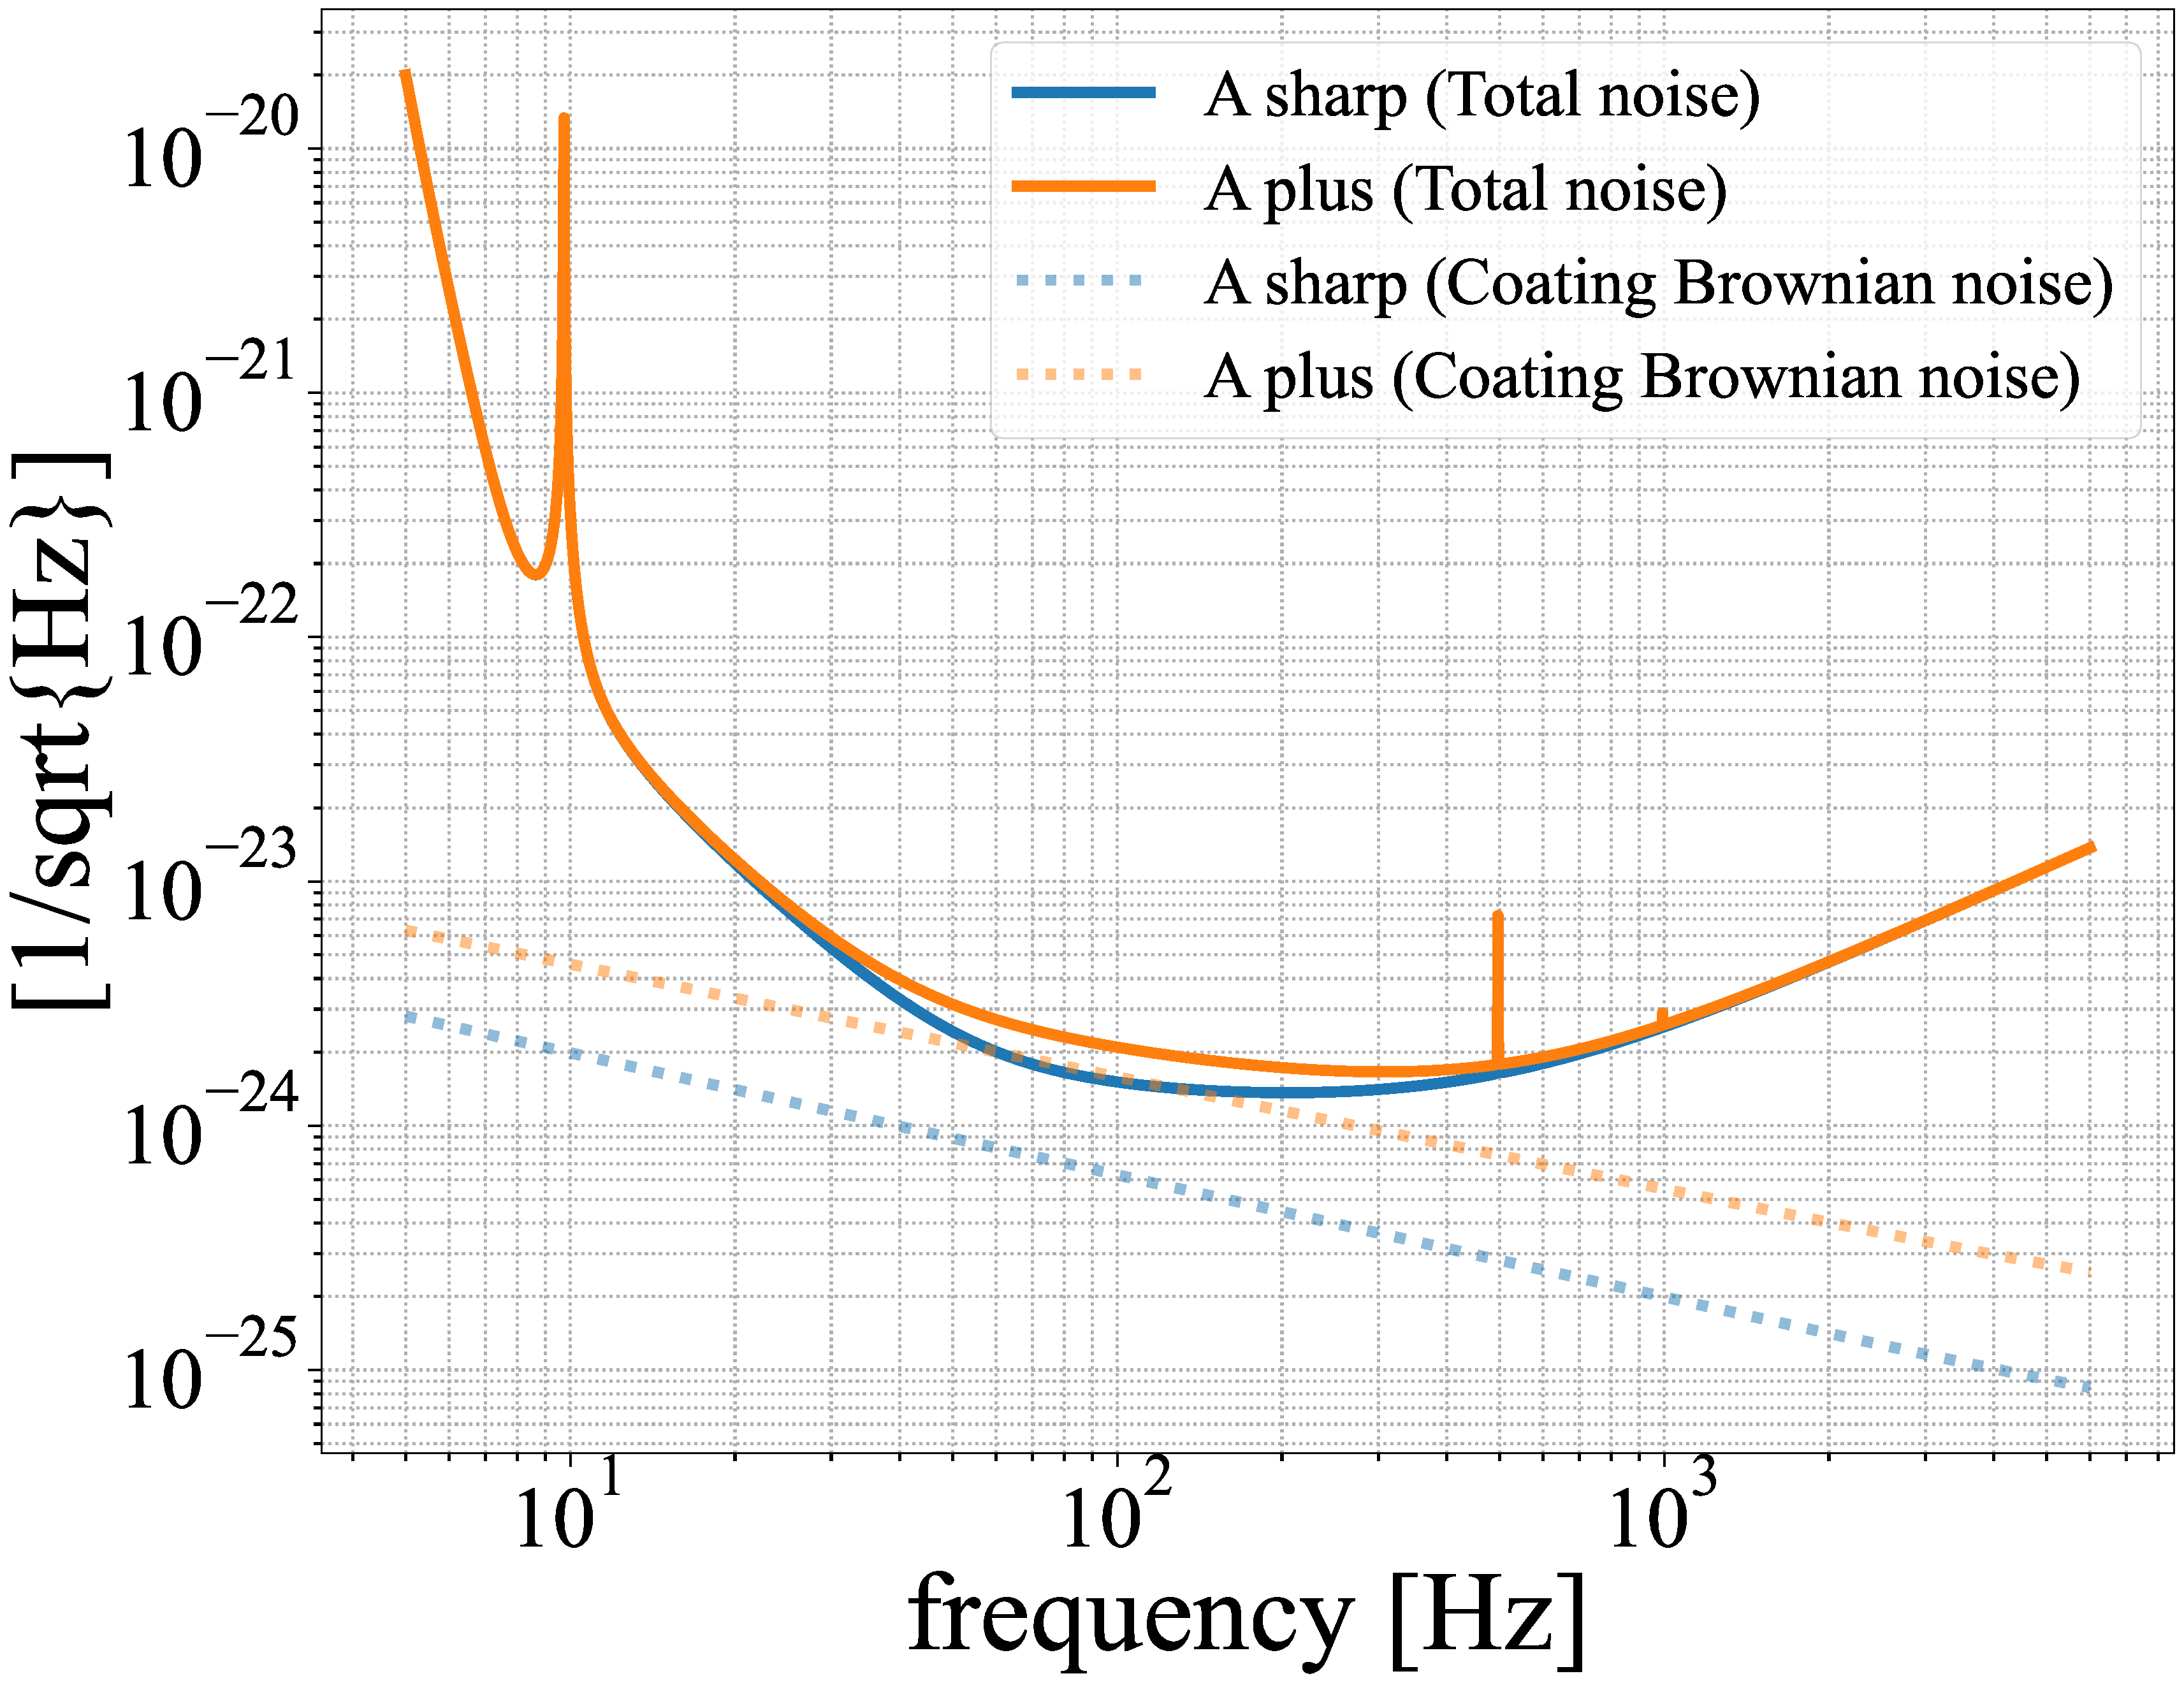
\includegraphics[width=\textwidth]{code/gwinc/aplus_CTN_compare.pdf}
    \end{center}
\caption{Comparison between $\siotao$ and $\gaas$/$\algaas$ coating brownian noise performance computed with a modified A+ GWINC model with coating parameters noted in ~\cite{dcc:asharp}.}
\label{fig:aligotncomp}
\end{figure}

%% Coating params table?
%\paragraph{$\siotao$ coating parameters} 
%Currently the LIGO interferometers deposit $\lambda$/4 stacks of silica and titania doped tantala on fused silica test mass substrates. Effective loss angle measurements \cite{harry:2006}
%
%\textbf{Current $\siotao$ elasticity params, power spectra, and strain spectral density (order of magnitude estimate)}
%
%\paragraph{$\gaas$/$\algaas$ coating parameters}
%%%Specific coating parameters for most promising $\algaas$ candidates? Chat with Steve. Or just mention parameters that are listed in Cole 2013
%\cite{cole:2013}
%
%%% Insert computed curves of the most precise and recent (effective) loss angle measurements (Nick Demos measurements?). More instructive to plot strain spectral density or displacement power spectra
%
%\noindent Currently thermal noise from the $\siotao$ optical coatings is the largest contributor of Brownian noise in LIGO compared to estimated substrate and suspension thermal noise \cite{harry:2006}. As of the end of O3, Brownian thermal noise is estimated to be ? orders of magnitude below the current sensitivity and it will prove to be the limiting source of noise as that sensitivity is increased with various other upgrades mitigating fundamental and technical noise. 
%%% Already mentioned in intro prior to this thermal noise section. Need to re-iterate in more detail?



As aLIGO approaches designed sensitivity, the thermal noise limit set by $\siotao$ HR coatings becomes an immediate limit to further improvements. Though there are proposals for the usage of alternative mirror coating solutions to push down this thermal noise limit for increased detector sensitivity \cite{harry:aigwd2019}. $\gaas$/$\algaas$ is a crystalline coating candidate showing promise for next generation detectors with reduced coating Brownian noise by a factor of 10, cooresponding to a potential strain reduction by a factor of 5 ~\cite{cole:2013} when compared to the current aLIGO coating thermal noise limit. 

\subsection{Coating Electro-optic Noise}
Applying crystalline HR mirror coatings to the core optics indiscriminately may introduce notable side effects; one being linear electro-optic noise of $\gaas$/$\algaas$ (dn/dE), also known as the Pockels effect ~\cite{abernathy:poster}. Although estimated to be nearly two orders of magnitude below the A$^\sharp$ strain noise floor ($\approx 10^{-26}$), direct measurement is still merited and adequately motivates a thorough study of electro-optical properties of $\gaas$/$\algaas$ coatings. The rest of this chapter discusses such a study by detailing: 1) birefringence in zincblende materials, 2) a preliminary estimation of differential phase noise of light reflected from a $\gaas$/$\algaas$ coating stack caused by electric field noise are computed while considering potential impacts to the current generation gravitational wave detectors, and 3) a short experimental optical cavity designed to interrogate an estimate of dn/dE from a calibrated differential length PDH locked signal with a normal electric field driven across a HR $\gaas$/$\algaas$ coating ``witness" sample.

\section{Birefringence in zincblende materials}
\subsection{The Indicatrix}\label{sec:indicatrix}
The two index solutions for a uniaxial crystal given a general plane wave with unit wave vector $\vec{k}$ can be found via a conveniant geometrical construction known as the ``index ellipsoid". 

\begin{figure}[ht!]
\begin{center}
\includegraphics[width=.85\textwidth]{figs/ALGAAS/indicatrix_alph.pdf}
\end{center}
\caption{A surface of uniform energy density ($U_E$) forming an ellipsoid in D-space for a generalized uniaxial crystal with general wavefront propogation indicated by a plane normal $\hat{k'}$ where the major and minor axes of the ellipse cross section indicate slow and fast axes $n_\beta$ and $n_\alpha$ respectively.}
\label{fig:genindtrx}
\end{figure}

The construction begins when considering a constant electric energy density ($U_e$) surface in the $\vec{D}$ space; which forms an ellipsoid: 

\begin{equation}\label{eq:lagr1}
\frac{D_x}{\varepsilon_x} + \frac{D_y}{\varepsilon_y} + \frac{D_z}{\varepsilon_z} = 2 U_e \varepsilon_o
\end{equation}
With redefined coordinates $(\vec{D}/\sqrt{2 U_e \varepsilon_o}) \rightarrow \vec{r}$ and setting $\varepsilon_i = n^2_i$:
\begin{equation}
\frac{x^2}{n_x^2} + \frac{y^2}{n_y^2} + \frac{z^2}{n_z^2} = 1
\end{equation}

This equation for the ellipsoid is known as the indicatrix. Given the co-planar solution demonstrated in \autoref{appendix:Diel_tensor}, we can impose the normal of the plane $\vec{r} \cdot \vec{s} = 0$:

\begin{equation}\label{eq:lagr2}
\vec{r} \cdot \vec{s} = x s_x + y s_y + z s_z = 0
\end{equation}
\autoref{eq:lagr1} and \autoref{eq:lagr2} both contribute constraints to the method of finding extrema using Lagrange multipliers for the function:
\begin{equation}
r^2 = x^2 + y^2 + z^2
\end{equation}
The Lagrangian ($\mathcal{L}$) with the introduced multiplers ($\lambda_1$, $\lambda_2$) then becomes:
\begin{equation}
\mathcal{L}(\vec{r},\vec{s},\lambda_1, \lambda_2) =
x^2 + y^2 + z^2 + \lambda_1 (xs_x + ys_y + zs_z) + \lambda_2 \bigg( \frac{x^2}{\varepsilon_x} + \frac{y^2}{\varepsilon_y} + \frac{z^2}{\varepsilon_z} - 1 \bigg)
\end{equation}
With the generated system of equations from the Lagrange multipler method ($\partial F_i/ \partial x_i = 0$, and $\partial F_j/ \partial \lambda_j$) where index $i =x,y,z$ and $j = 1,2$ we obtain a system of 3 equations:
\begin{equation}
i \bigg(1-\frac{r^2}{\varepsilon_{i}} \bigg) + s_{i} \bigg(\frac{x s_x}{\varepsilon_x} + \frac{y s_y}{\varepsilon_y} + \frac{z s_z}{\varepsilon_z} \bigg) = 0
\end{equation}
The result is verified when substituting $r \rightarrow \frac{\vec{D}}{\sqrt{\vec{E} \cdot \vec{D} \varepsilon_o}}$ back which recovers \autoref{eq:modelec}.
\\
\subsection{\texorpdfstring{$\gaas$}{gaas} and \texorpdfstring{$\algaas$}{algaas} crystal classification}
$\gaas$ as well as $\algaasgen$ are both within the $F\bar{4}3m$ space group. Crystals of this space group are commonly known as zincblende crystals; a common crystal configuration named after zinc sulfide (ZnS). Also categorized as a cubic crystal, their crystallographic structure displays linear optical isotropy when stress free and no DC and/or slowly varying electric fields are present~\cite{boyd:2008}. 

\begin{figure}[!ht]
\begin{center}
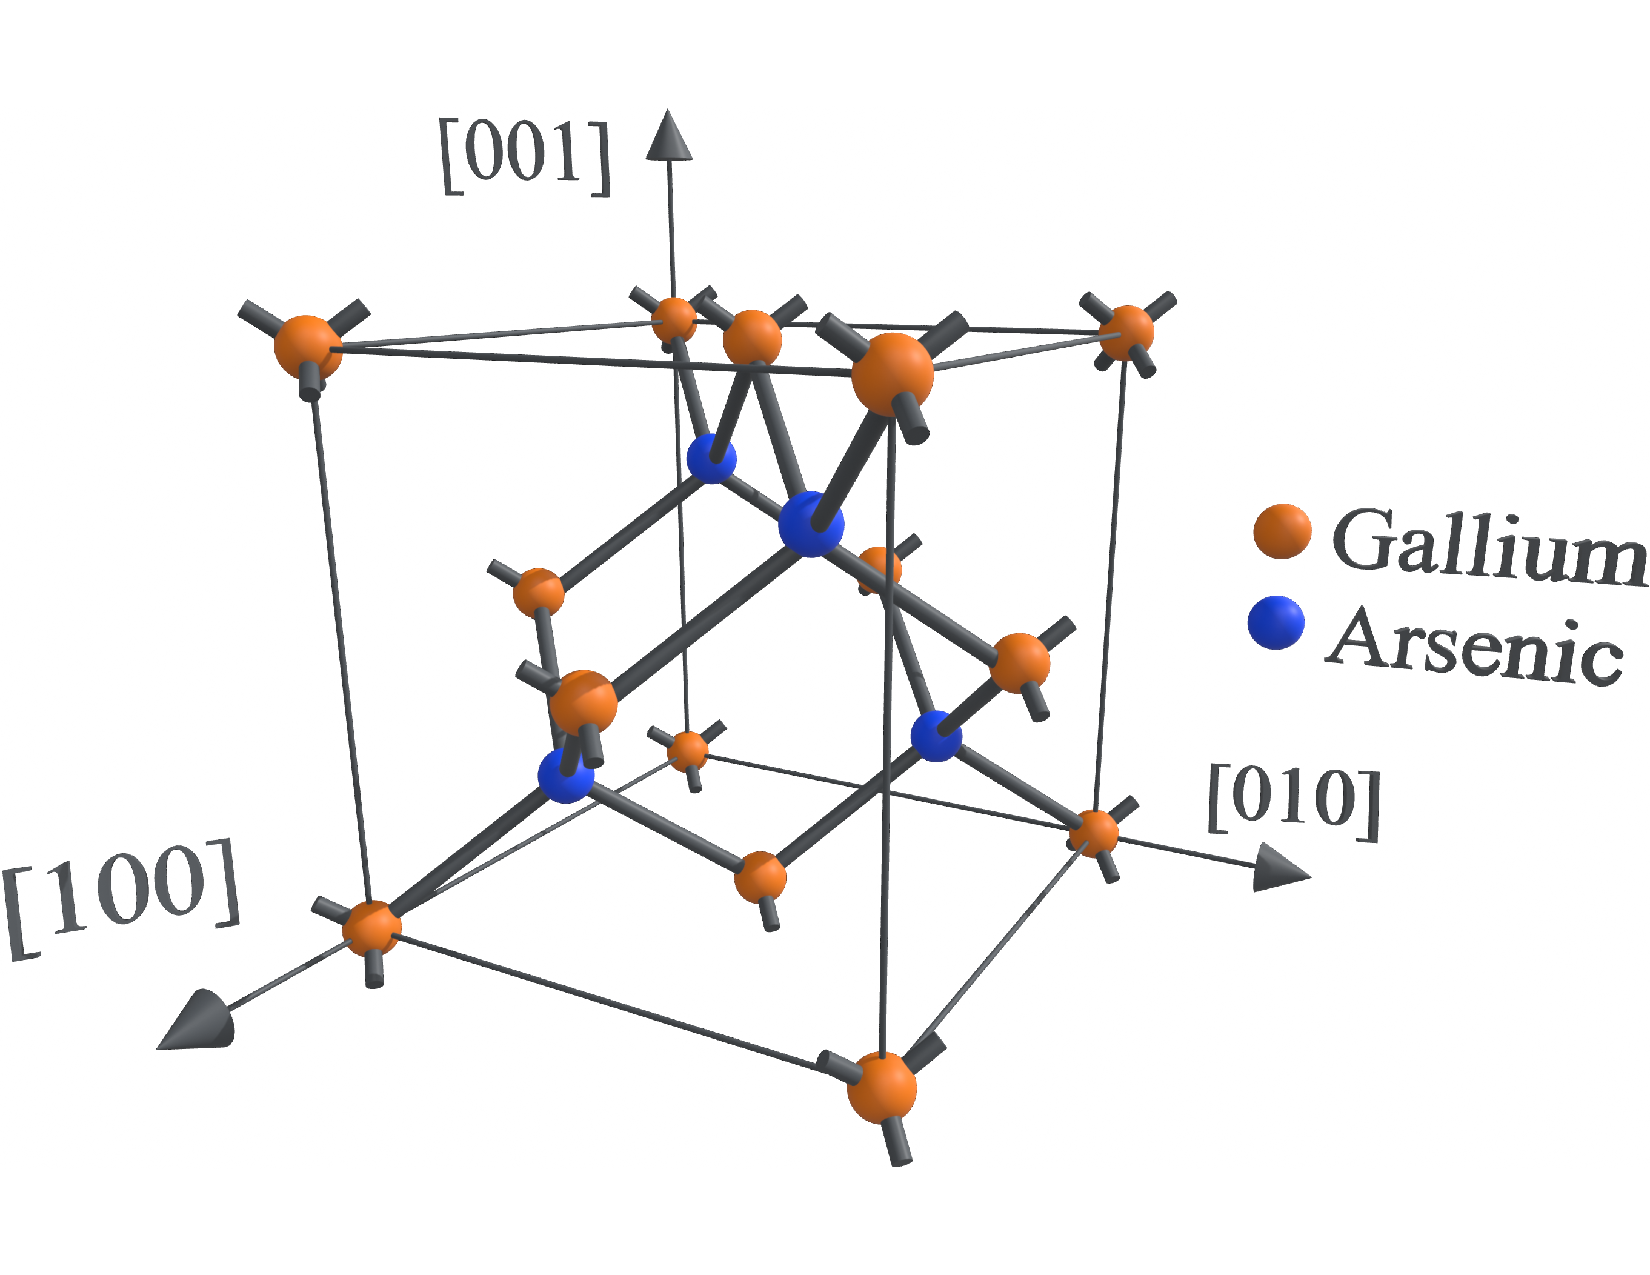
\includegraphics[width=.5\textwidth]{figs/ALGAAS/gaas_unit_cell_mi.pdf}
\caption{The unit cell of gallium arsenide (GaAs) with associated miller indices as coordinate axes}
\end{center}
\label{fig:gaasuc}
\end{figure}

Zincblende structures, like the crystalline materials in question can exhibit birefringent properties when under influence of mechanical stresses and static / low-frequency electric fields ($E_\mathrm{STLF}$); characterized by photoelastic and electro-optic effects respectively. For realistic mirror coatings, heteroepitaxial bonding between $\gaas$/$\algaas$ layers (potentially from a noticiable difference in lattice cell constant) may produce an intrinsic strain within the HR stack and can lead to the existence of a static non-negligible birefringence throughout the coating layers \cite{cole:2016, adachi:1985}.

\subsection{Linear electro-optic effect (Pockel's effect)}
For non-centrosymmetric crystalline media there exists a non-zero rank 2, $6 \times 3$ tensor ($r_{ij}$) connecting low-frequency \footnote{``low frequency'' meaning orders of magnitude smaller relative to an optical field} electric fields $\vec{E_{STLF}}(f) = [E_x(f), E_y(f), E_z(f)]$ directly to the \hyperref[sec:indicatrix]{indicatrix} ~\cite{yariv,nye}:
\begin{equation}
  \left[ {\begin{array}{c}
   \big( \frac{1}{\Delta n ^2 } \big)_1 \\
   \big( \frac{1}{\Delta n ^2 } \big)_2 \\
   \big( \frac{1}{\Delta n ^2 } \big)_3 \\
   \big( \frac{1}{\Delta n ^2 } \big)_4 \\
   \big( \frac{1}{\Delta n ^2 } \big)_5 \\
   \big( \frac{1}{\Delta n ^2 } \big)_6 \\
  \end{array} } \right]
  =
%
 \left[ {\begin{array}{ccc}
   r_{11} & r_{12} & r_{13}\\
   r_{21} & r_{22} & r_{23}\\
   r_{31} & r_{32} & r_{33}\\
   r_{41} & r_{42} & r_{43}\\
   r_{51} & r_{52} & r_{53}\\
   r_{61} & r_{62} & r_{63}\\
  \end{array}} \right]
 %
 \left[{\begin{array}{c}
   E_x (f)\\
   E_y (f)\\
   E_z (f)\\
 \end{array}} \right]
\end{equation}

\noindent The $i$ index runs over the terms in the indicatix equation:
\begin{equation}
\bigg(\frac{1}{\Delta n_x^2} \bigg) x^2\ + \bigg(\frac{1}{\Delta n_y^2} \bigg) y^2 + \bigg(\frac{1}{\Delta n_z^2} \bigg) z^2 + 2 \bigg(\frac{1}{\Delta n_{xz}} \bigg)xz + 2 \bigg(\frac{1}{\Delta n_{yz}} \bigg)yz + 2 \bigg(\frac{1}{\Delta n_{xy}} \bigg)xy = 1
\end{equation}

%%Detail on some prior knowledge of $f \leq f_\mathrm{max}$? (Pockels cell specs?)

\subsubsection{\texorpdfstring{$r_{ij}$}{rij} for zincblende crystals (\texorpdfstring{$r_{\bar{4}3m, ij}$}{r43})}

The form of the electro-optic tensor for zincblende crystals (including $\gaas$ and $\algaas$) reduces such that $r_{ij} = r_{41} = r_{52} = r_{62} \neq 0$ with all other terms being zero:

\begin{equation}
r_{\bar{4}3m,ij} =
 \left[ {\begin{array}{ccc}
  0 & 0 & 0\\
  0 & 0 & 0\\
  0 & 0 & 0\\
  r_{41} & 0 & 0\\
  0 & r_{52} & 0\\
  0 & 0 & r_{63}\\
 \end{array}} \right]
\end{equation}

\noindent Where $r_{41} = r_{52} = r_{63}$

\subsection{New principal (electro-optic) dielectric axis for zincblende structures}
In general the principle dielectric axes of the new ellipsoid do \textbf{not} coincide with the axes of the ellipsoid of the unperturbed crystal. The form of the index ellipsoid for a zincblende crystalline material accounting for the electro-optic tensor and some generalized DC electric field $\vec{E}$ expressed in terms of the crystallographic axes is given by:
\begin{equation}\label{eq:zindicatrix}
\bigg(\frac{1}{n_o^2} \bigg) x^2\ + \bigg(\frac{1}{n_o^2} \bigg) y^2 + \bigg(\frac{1}{n_o^2} \bigg) z^2  + 2r_{41} E_{x} yz + 2r_{41} E_{y} xz + 2r_{41}E_{z} xy= 1
\end{equation}

\noindent Where we have set $n_x = n_y = n_z = n_o$ for zincblende structures. Visualizing the above as a tensor:

\begin{equation}
\left[ {\begin{array}{ccc}
   \big( \frac{1}{n_o ^2} \big)& r_{41}E_{x} & r_{41} E_{y}\\
   r_{41}E_{x} & \big( \frac{1}{n_o ^2} \big) & r_{41} E_{z}\\
   r_{41} E_{y} & r_{41} E_{z} & \big( \frac{1}{n_o ^2} \big)\\
\end{array}} \right]
\end{equation}

\subsection{The photoelastic effect}

General stresses and strains of a material may also cause transformations to the indicatrix connected by the rank 4 elasto-optical tensor $p_{i j k l}$:

\begin{equation}
 \bigg( \frac{1}{\Delta n^2} \bigg)_{ij} = p_{ijkl} \epsilon_{kl}
\end{equation}

\noindent Where the strain ({\boldmath$\epsilon$}) relates to stress ({\boldmath$\sigma$}) using the generalized Hooke's law: 
%\begin{equation}\label{eq:indicgen_stress2strain}
%	\epsilon_{\alpha \beta} = r_{\gamma \alpha \beta}E_{\alpha} + s_{\alpha \beta \gamma \theta } \sigma_{\gamma \theta}
%\end{equation}
% elasto-optic ($p_{ij \alpha \beta}$) tensor to the stress tensor ($\epsilon_{\alpha \beta}$) via stress-strain / piezoelectric relations:
\begin{equation}\label{eq:genhookeslaw} 
 \begin{split}
	 \epsilon_{ij} = K_{ijkl} \sigma_{kl}
	 \\
	 \sigma_{ij} = C_{ijkl} \epsilon_{kl}
 \end{split}
\end{equation}
A connection is also formed between the elasto-optical tensor ({\boldmath$p$}) to the piezo-optical tensor ({\boldmath$\pi$}): 
\begin{equation}\label{eq:indicgenelastooptical}
 \begin{split}
	p_{ijkl} = \pi_{ijkl} C_{klrs}
	\\
	\pi_{ijrs} = p_{ijrs} K_{rskl}
 \end{split}
\end{equation}

\subsection{The generalized indicatrix}
Both forms of the induced birefringence (electro-optic and photo-elastic) can be incorportated into a condensed form \cite{nye}:

\begin{equation}\label{eq:indicgen}
	\bigg( \frac{1}{\Delta n^2} \bigg)_{ij} = r_{ijk}E_k + p_{ijkl} \epsilon_{kl}
\end{equation}


%%New principal dielectric axes for zincblende structures (zinblende photoelastic tensor, zincblende electro-optic tensor)

\section{Electro-optic noise of a \texorpdfstring{$\gaas$}{gaas} / \texorpdfstring{$\algaas$}{algaas} stack}
A comprehensive survey of relevant birefringent properties of a HR $\gaas$/$\algaas$ mirrorstack is due, and for this body of work includes: 1) crystal coordinate considerations when asserting an optical axis on a highly reflective crystalline stack manufactured by the Thorlabs crystalline coatings division, 2) citations of coating parameters and observed intrinsic birefringence from the highly reflective coating stack in question, 3) analysis of the differential electro-optic effect on the phase of a reflected beam, and 4) estimating the the differential phase noise in LIGO based on preliminary electric field measurements measured at LHO.

\subsection{Static Birefringence / Miller indices from a HR \texorpdfstring{$\gaas$}{gaas} / \texorpdfstring{$\algaas$}{algaas} coating}

\begin{figure}[!ht]
    \centering
	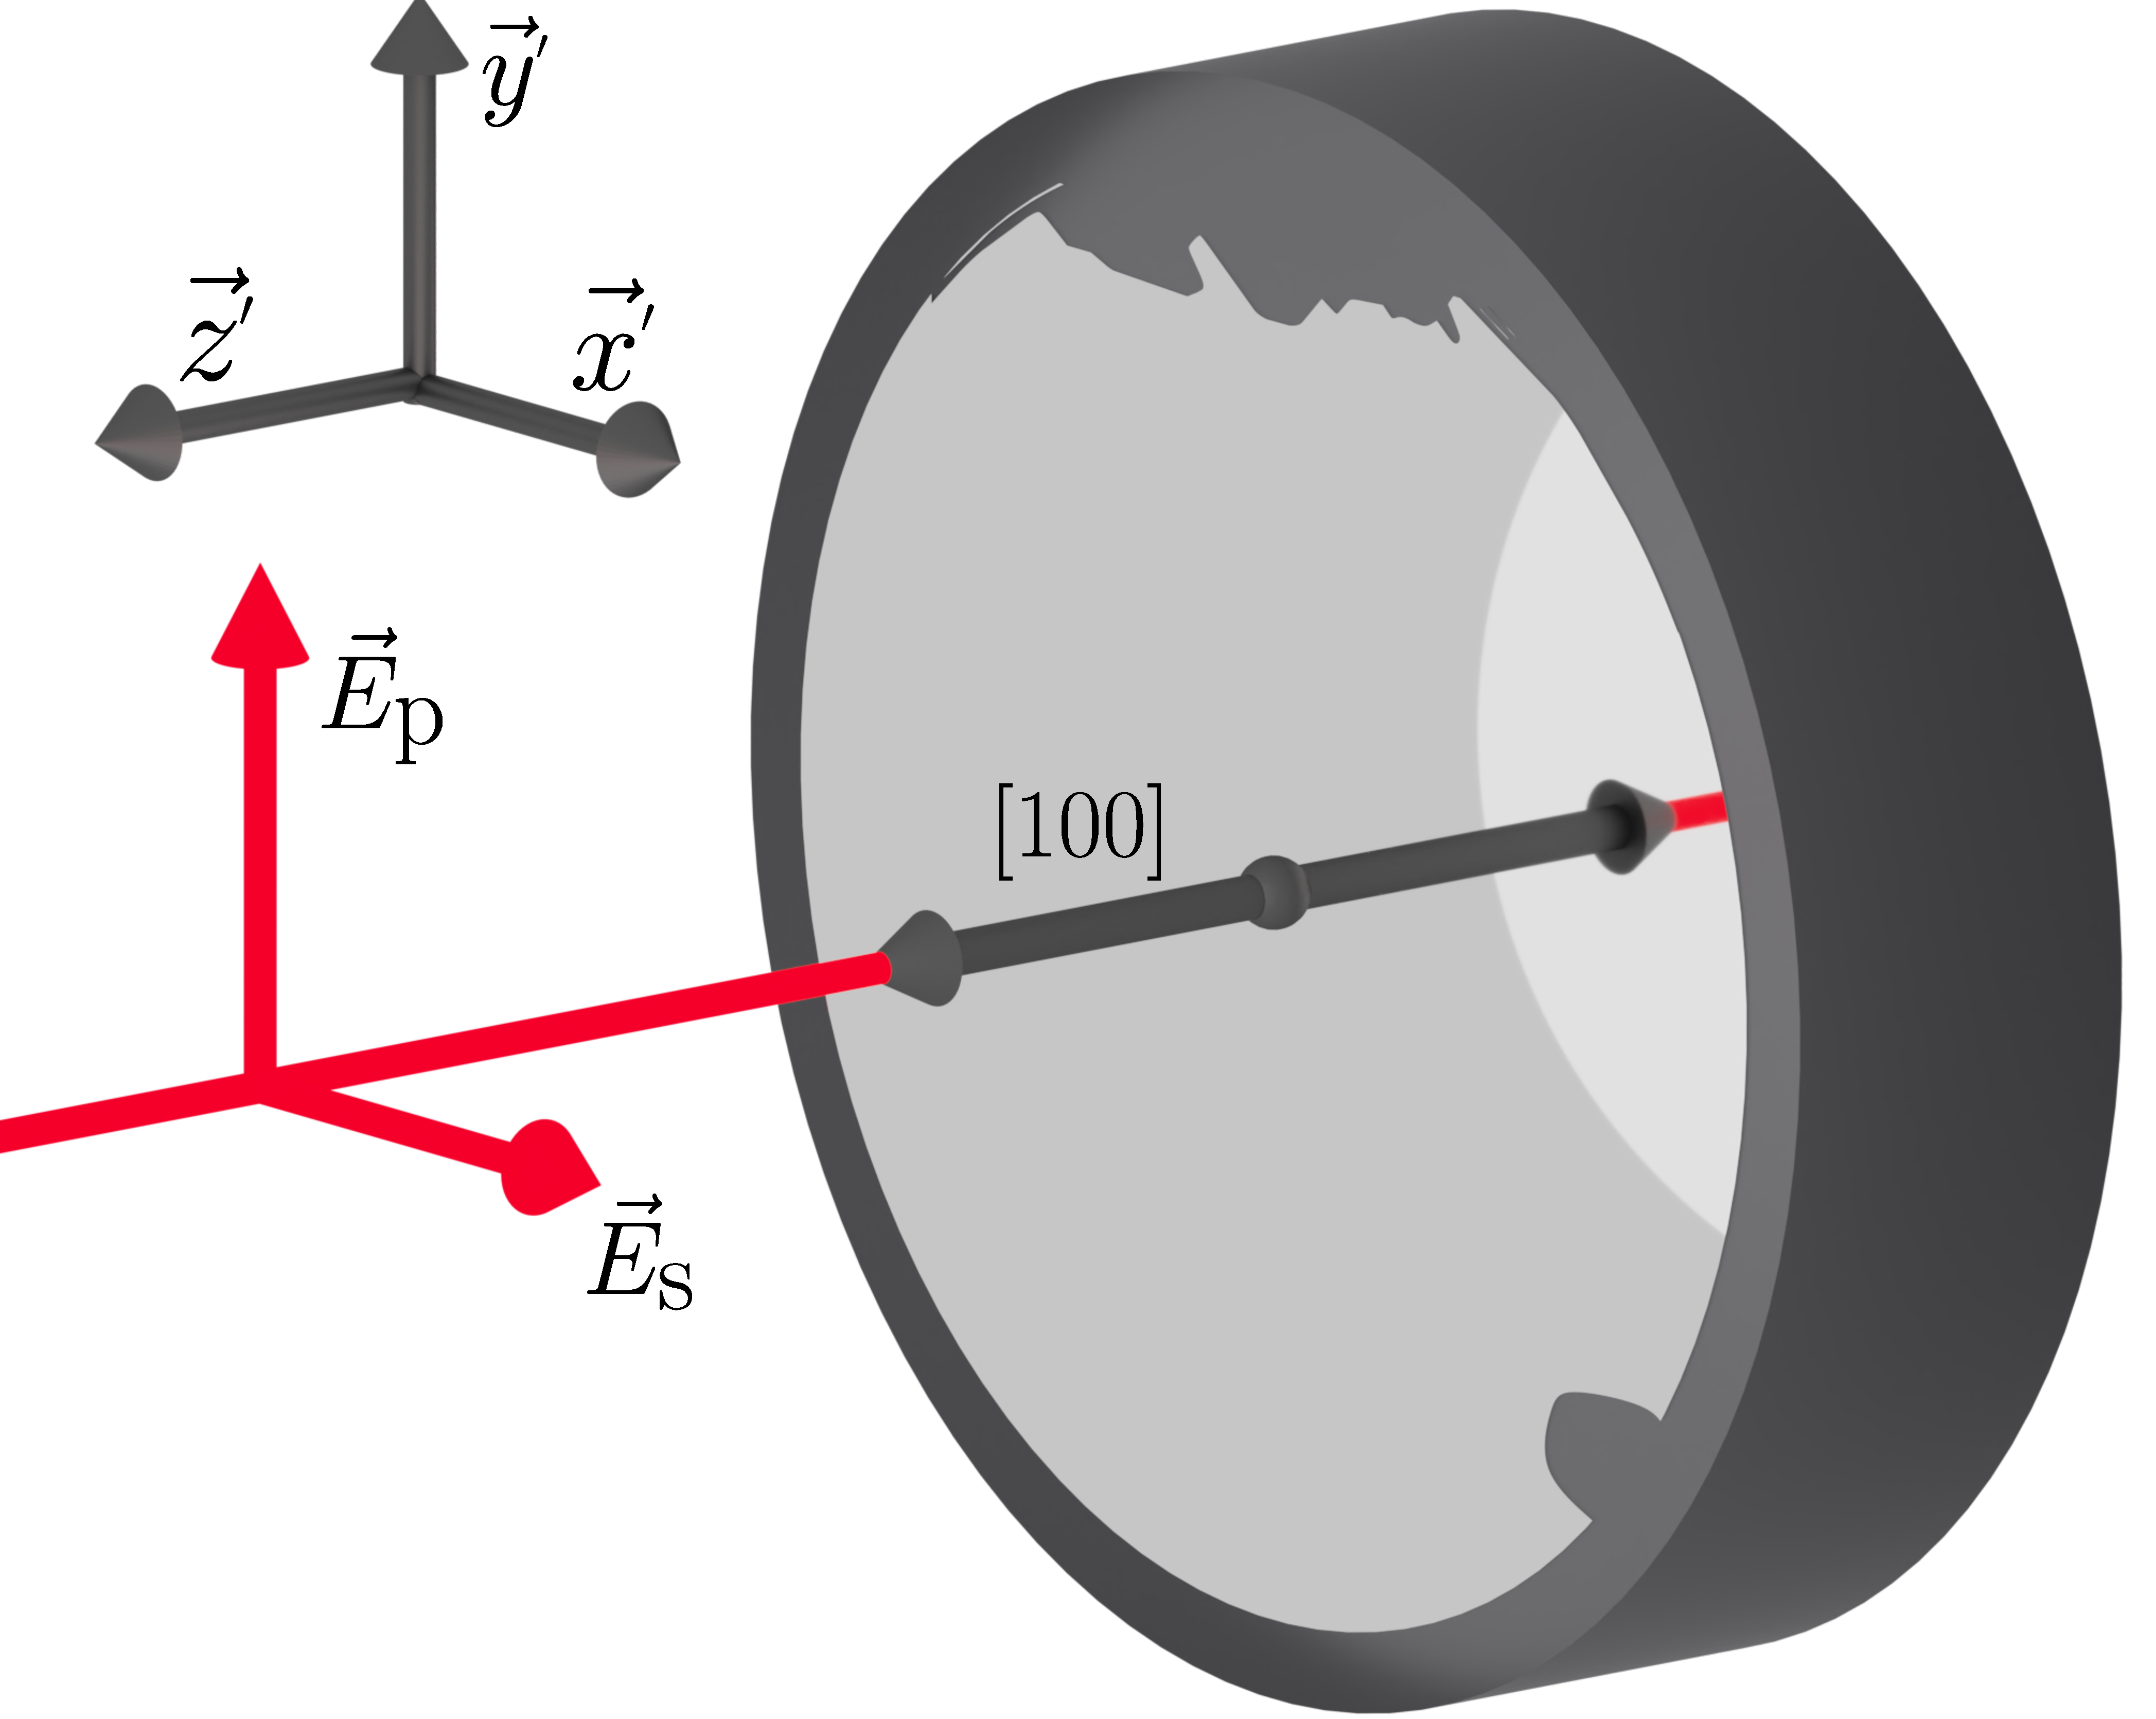
\includegraphics[width=.6\textwidth]{figs/ALGAAS/laser_mirror_algaas_coat_defect_coords.pdf}
	\caption{The beam propogation axis with respect to the $\gaas$/$\algaas$ crystal axis. The axis formed by the [100] plane normal is drawn parallel with the beam axis (z-axis) and the polarizations of incident and reflected beam oscillate along vectors within the plane formed by the normal of that axis. The topmost coordinate axis triad is drawn to depict world vectors that can help visualize the plane of computed eigenvectors. Depicted here are also defects at the top and bottom right of the coating due to overhandling but do not effect the results of this study.}
\label{fig:algaas_coord_defect}
\end{figure}

\noindent Thorlab's crystalline coatings division grows their HR crystalline optical coating such that the coating surface is drawn out in the $[100]$ plane, meaning that beam with a wavevector along the optical (z) axis draws a parallel line to the normal of said plane. Therefore since the beam's polarized E-field oscillates only within that plane, any differential splitting of the beam polarization occurs solely between rotated $[010]$ and $[001]$ axes. This allows us to restrict our interest to a field where $E_{z} \neq 0$ and $E_x = E_y =0$ and compute the eigenvalues ($\lambda^{*}_{x',y',z'}$ / eigenpolarizations ($\vec{x'}, \vec{y'}, \vec{z'}$) which lead us to the relevant eigenindices ($n_{x',y'})$ \footnote{There may appear to be an inconsistency between the miller indices and optical axes, but because of the isotropy of zincblende crystals prior to the field perturbation coordination of these axes is not quite relevant}:

\begin{equation}
    \begin{aligned}
    	\lambda_{x'} & = \big( \frac{1}{n_o ^2} - r_{41} E_z \big) \\
	\lambda_{y'} & = \big( \frac{1}{n_o ^2} + r_{41} E_z \big) \\
	\lambda_{z'} &  = \frac{1}{n_o ^2}
    \end{aligned}
\end{equation}

\noindent And the principal axes / eigenpolarizations are found when solving for the eigenvectors:

\begin{equation}
    \begin{aligned}
	\vec{x'} & = \frac{1}{\sqrt{2}}\;(0, -1, 1) \\ 
	\vec{y'} & = \frac{1}{\sqrt{2}}\;(0, 1, 1) \\
	\vec{z'} & = (1, 0, 0) \\
    \end{aligned}
\end{equation}

\begin{equation}
    \lambda_{x'}\; x'^2 + \lambda_{y'}\; y'^2 + \lambda_{z'}\; z'^2 =1
\end{equation}

\noindent The eigenindices ($n_\alpha = n_{x'}$, $n_\beta = n_{y'}$) are therefore:

\begin{equation}
    \begin{aligned}
	n_{x'} & = \sqrt{\lambda_{x'}} & = \sqrt{\frac{1}{n_o ^2} - r_{41} E_z} \\
	n_{y'} & = \sqrt{\lambda_{y'}} & =  \sqrt{\frac{1}{n_o ^2} + r_{41} E_z}
    \end{aligned}
\end{equation}



\noindent And with $n_o r_{41} E_z << 1$:

\begin{equation}
    \begin{aligned}
	n_{x'} & \approx  n_o + \frac{1}{2} n_o^3 r_{41} E_z \\
	n_{y'} & \approx n_o - \frac{1}{2} n_o^3 r_{41} E_z    
    \end{aligned}
\end{equation}

\subsection{Electro-optic coupling to the reflected phase of a HR mirror coating}
%With our chosen beam axis, the influence of an isotropic white noise field ($E_N = [E_{Nx},E_{Ny},E_{Nz}]$) is considered:

%\begin{equation}
% \left[ {\begin{array}{ccc}
%   \big( \frac{1}{n_o ^2} \big)& r_{41}E_{Ny} & r_{41} E_{Nx}\\
%   r_{41}E_{Ny} & \big( \frac{1}{n_o ^2} \big) & r_{41} E_{Nz}\\
%   r_{41} E_{Nx} & r_{41} E_{Ny} & \big( \frac{1}{n_o ^2} \big)\\
%  \end{array}} \right]
%\end{equation}

%\noindent Assuming $E_N$ is small, the indicatrix change of $E_{Nx}$ and $E_{Ny}$ relative to $E_{Nz}$ (as seen by the beam polarization) will be small ($r_{41}E_{N(x/y)} \ll r_{41}E_{Nz}$). After diagonalizing with relevant terms \footnote{Note that the form of the tensor is still in the crystal coordinates but the $E_n$ terms are placed in the tensor such that their directions align with beam axis coordinates.} in the tensor, we are left with the following eigenindices:
%
%\begin{equation}
%\begin{aligned}
%n_x' & = n_o - r_{41}E_{Nz} \\
%n_y' & = n_o + r_{41}E_{Nz}
%\end{aligned}
%\end{equation}

%How the modulation of the phase of the carrier field is dependent on the orientation of its wave vector with respect to the crystal structure, the modulating electric field direction and strength, (other items to discuss in terms of introducing the effect)
%% For GaAs @ $10.6\mu$ $r_{41} = 1.6 \times 10^{-12}$ [m/V]
%% Adachi estimate for $\mathrm{Al_{x}Ga_{1-x}As}$?
%% Relevant eigenpolarizations, non-optical field $E_y = E_z = 0$?}
%% FIGURE: SUB1 Transformed indicatrix (Before and after $E_x$)
%% FIGURE: SUB2 Ellipse cross section. New eigenpolarizations and corresponding indices and their influence on incident field (Marty's result)

\subsubsection*{Analytic estimate}
Fejer and Bonilla takes on an analytical approach to finding the impact of the electric field to the change in phase of the light through a crystalline anisotropic thin film ($\lambda/4$) stack. The construction builds off of a pre-defined derivation of thermo-optic noise calculations for the HR stack and assuming a large enough number of high-low index coating pairs~\cite{bonillafejer, fejer_estimate}:

\begin{equation}
    \bigg| \frac{\partial \phi}{\partial E} \bigg| = - \pi \frac{r_{41}}{2}(n_\mathrm{high} n_\mathrm{low} ^2 + n_\mathrm{low} n_\mathrm{high} ^2) \frac{n_\mathrm{high}}{n_\mathrm{low}}
\end{equation}

With $n_\mathrm{low} = n_\algaas = 2.9369$, $n_\mathrm{high} = n_\gaas = 3.4786$, and $r_{41} = -1.33 \times 10^{-12}$

The estimated differential phase from the electro-optic effect with a 1064nm E-field propogating along the [110] axis of the HR $\gaas / \algaas$ stack:

$$
\bigg| \frac{\partial \phi}{\partial E} \bigg| = 4.0253 \times 10^{-12} \; \frac{[\mathrm{rad}]}{[\mathrm{V}/\mathrm{m}]}
$$
%\begin{equation}
%\hat{\phi}' = \frac{\pi n_1 z}{1-z^2}(z^{2N} -1) \frac{z^{2N} \frac{(n_f)^2}{n_2 n_3}(n_2 \kappa_{\gamma 2} + n_3\kappa_{\gamma 3}) - (n_2 \kappa_{\gamma 3} + n_3\kappa_{\gamma 3})}{(n_1)^2 -(n_f)^2 z^{4N}}
%\end{equation}

%with $z = \frac{n_2}{n_3}$
%and
%$
%\kappa_{\gamma j} = \frac{d}{d \gamma} \mathrm{log}(n_j h_j)|_{\gamma =\gamma_{O}} \bigg(\frac{\hat{n}_j'}{\hat{n}_j} +\frac{\hat{h}_j'}{\hat{h}_j} \bigg)
%$

%With $\kappa$ being a scalar parameter.
%%FIGURE: Cross sectional view of multilayer coating

\begin{figure}[!ht]
	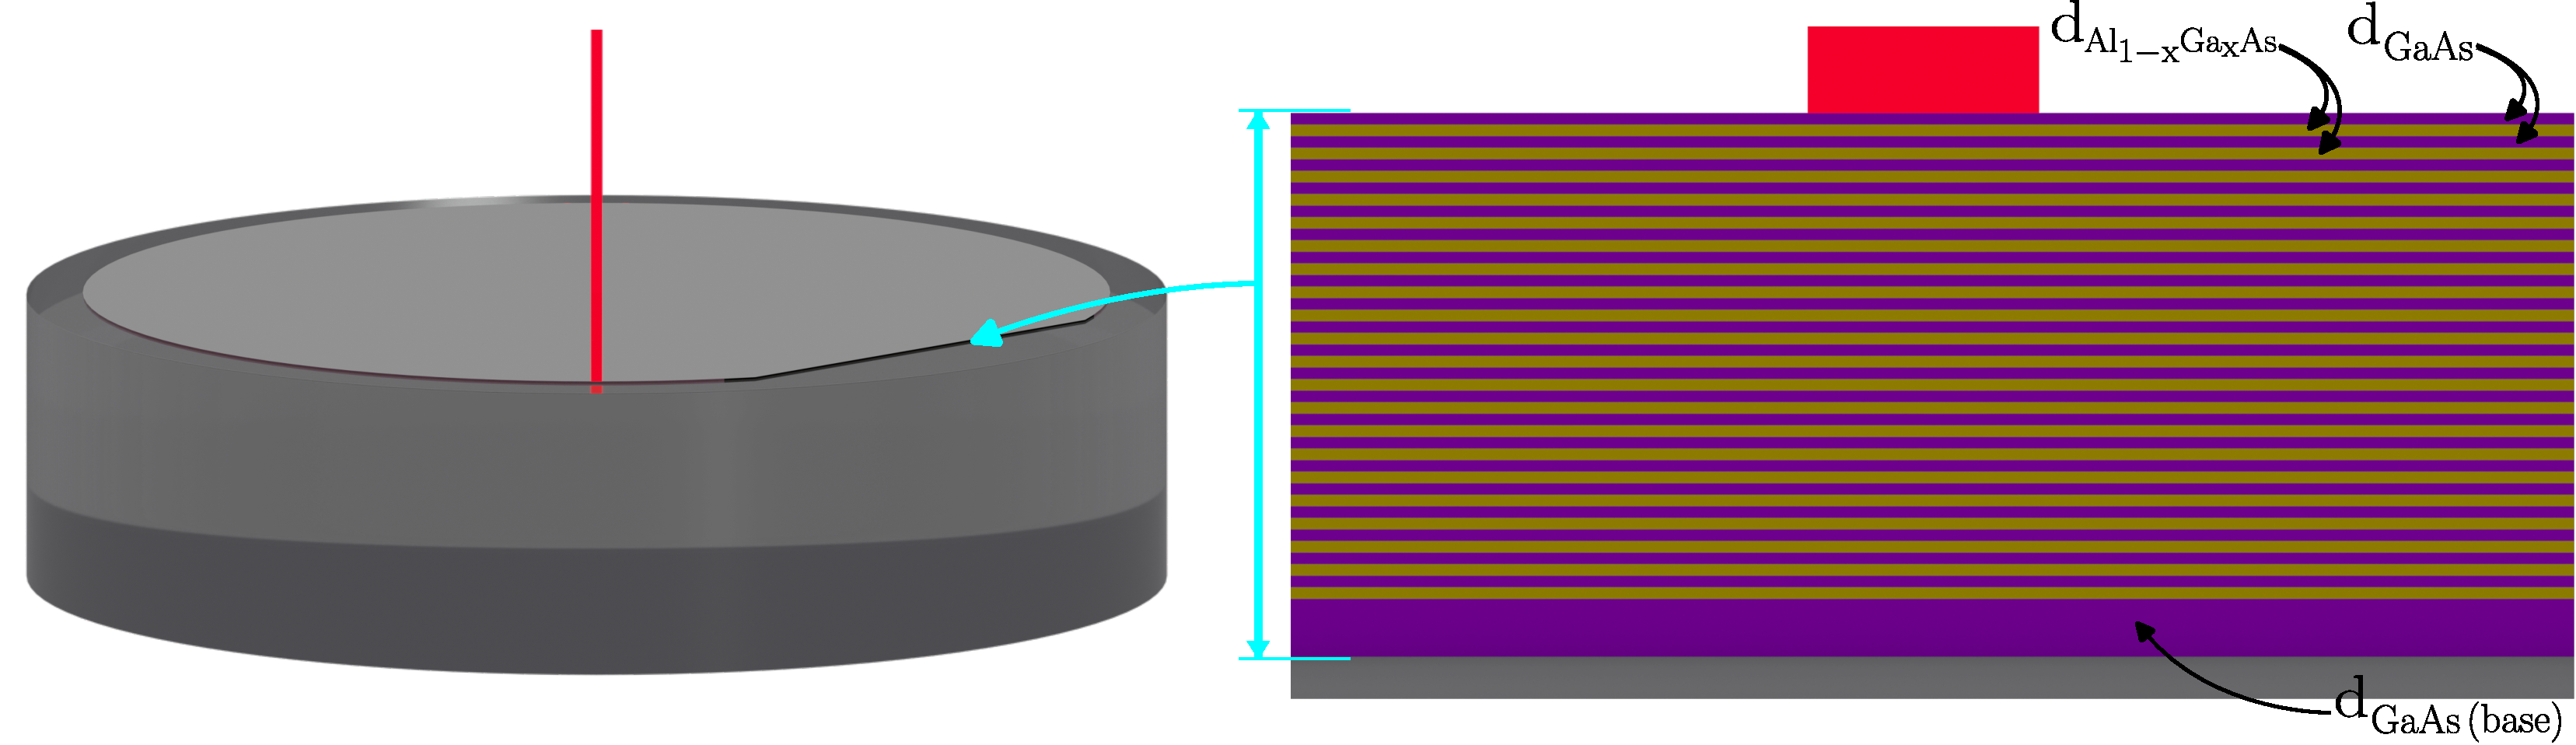
\includegraphics[width=\textwidth]{figs/ALGAAS/ALGAAS_HR_layers_ann.pdf}
\caption{The beam propogation axis ($\vec{S}$, $[-100]$) with respect to the $\gaas$/$\algaas$ crystal axes. The axis formed by the [100] plane normal is drawn parallel with the beam axis (z-axis) and the polarizations of incident and reflected beam oscillate along vectors within the plane formed by the normal of that axis. Usually, these coatings made by Thorlab's crystalline mirror coatings division is grown with a flat indicating a line within the [0-11] plane; where the plane normal points towards the sample center.}
\label{fig:HRlayers}
\end{figure}


\subsubsection*{Numerical estimate}\label{algaas_numericalestimate}

In the appendix of \cite{ballmer:2015} Ballmer constructs a coating layer transfer function for a given coating layer k with index $n_k$, and thickness $d_k$, defining right and left propogating modes $\psi^{R,L}$ repsectively:
$$
  \left[ {\begin{array}{c}
   \psi^\mathrm{R} \\
   \psi^\mathrm{L} \\
  \end{array} } \right]_{k+1}
  =
%
Q_k D_k
%
 \left[{\begin{array}{c}
   \psi^\mathrm{R} \\
   \psi^\mathrm{L} \\
 \end{array}} \right]
$$
\noindent $D_k$ applies the phase ($\phi_k = 4\pi n_k d_k /\lambda_0$) from a given coating layer, and $Q_k$ applies the transfer function between high-low/low-high index layers transition:

\begin{equation}
D_k =
\left[ {\begin{array}{cc}
  e^{-i \phi_k / 2}& 0\\
 0 & e^{i \phi_k / 2}\\
\end{array} } \right]
\end{equation}

\begin{equation}
Q_k = \frac{1}{2n_{k+1}}
\left[ {\begin{array}{cc}
  n_{k+1} + n_k & n_{k+1} - n_k\\
 n_{k+1} - n_k & n_{k+1} + n_k\\
\end{array} } \right]
\end{equation}
\noindent Defining a HR coating stack, the total transfer matrix from vaccum $Q_0$ to the $N$th coating layer is:
\begin{equation}
	M = Q_N D_N ...Q_k D_k...Q_1D_1Q_0
\end{equation}
\noindent And the partial derivative at the kth coating layer is:

\begin{equation}
	\label{eq:partialM}
	\frac{\partial M}{\partial \phi_k} = Q_N D_N ...Q_{k} \begin{bmatrix} e^{-i \phi_k /2} & 0 \\ 0 & e^{i \phi_k/2} \end{bmatrix} \begin{bmatrix} -i /2 & 0 \\ 0 & i/2 \end{bmatrix} Q_{k-1} D_{k-1}...Q_1D_1Q_0
\end{equation}

\noindent The above representing a collective differential phase manifesting as a sum of these phase components. This explicit perturbed phase at the kth layer for the electro-optic effect ($\partial n_k/\partial E$) is found when:
\begin{equation}\label{eq:EOphasekdiff}
	\frac{\partial \phi_k}{\partial E} = \frac{4 \pi d_k}{\lambda} \frac{\partial n_k}{\partial E} = \pm \frac{ 2 \pi}{\lambda} n_k^3 d_k r_{41,k}
\end{equation}
\noindent Where the electro-optic coefficients $r_{41}$ for $\gaas$ and $\algaasgen$ \cite{suzuki:1984, adachi:2012, adachi:1985}:
\begin{equation}
\begin{aligned}
	& r_{41, \gaas} =  -1.33 \times 10^{-12} & [\mathrm{m} / \mathrm{V}]
	\\ 
	& r_{41, \algaasgen}  = - (1.33 - 0.45x) \times 10^{-12} &  [\mathrm{m}/\mathrm{V}]
\end{aligned}
\end{equation}
\noindent Rather than tagging on the phases individually, an easier computation is found when relying on the relationship between the transmission ($t$) and reflectivity ($r$) to a general transfer matrix (in our case $M$):
$$
	\begin{bmatrix} 1 \\ r \end{bmatrix} \begin{bmatrix} M_{11} & M_{12} \\ M_{21} & M_{22} \end{bmatrix} = \begin{bmatrix} t \\ 0\end{bmatrix}
$$
\noindent And using this relation, differentiating the reflectivity with respect to $\phi_k$:
$$
	\frac{\partial r}{\partial \phi_k} = - \bigg( \frac{1}{M_{21}} \frac{\partial M_{21}}{\partial \phi_k} - \frac{1}{M_{22}}\frac{\partial M_{22}}{\partial \phi_k} \bigg) \frac{M_{21}}{M_{22}}
$$
\noindent The differential reflectivity is normalized by the total reflectivity and taking the imaginary component as noted in~\autoref{eq:partialM}: 

\begin{equation}
	\frac{\partial \phi_c}{\partial \phi_k}  = \mathrm{Im} \bigg(\frac{1}{r} \frac{\partial r}{\partial \phi_k} \bigg) =  \bigg( \frac{1}{M_{21}} \frac{\partial M_{21}}{\partial \phi_k} - \frac{1}{M_{22}}\frac{\partial M_{22}}{\partial \phi_k} \bigg) 
\end{equation}

\noindent The impact of a differential electric noise field ($E_\mathrm{STLF}$) on $M$ due to the electro-optic effect on the kth layer, we use the chain rule:

\begin{equation}
	\bigg| \frac{\partial \phi_c}{\partial  E_\mathrm{STLF}} \bigg| =  \bigg| \frac{\partial \phi_c}{\partial \phi_k}  \frac{\partial \phi_k}{\partial E} \bigg|
\end{equation}

The coating to be studied consists of 36 $\lambda$/4  thick layers of $\gaas$ interspersed with 35 layers of $\lambda$/4 thick $\algaas$. $\gaas$ forms the top and bottom layer to prevent oxygen absorption from the AlGaAs layer. The $\gaas$ layers have an index of $n_{\gaas} = 3.480$ and a thickness of $\Delta d_{\gaas} = 76.43$ nm while the low index $\algaas$ layers are $n_{\algaas} = 2.977$ with thickness $\Delta d_{\algaas} = 89.35$ nm. With the constructed matrices, we apply these parameters and compute a differential phase of:

\begin{equation}
    \bigg| \frac{\partial \phi_c}{\partial  E_\mathrm{STLF}} \bigg|  = 3.9 \times 10^{-11}\; \frac{[\mathrm{rad}]}{[\mathrm{V}/\mathrm{m}]}     
\end{equation}

%High Index:  GaAs, n=3.480, layer thickness is 76.43 nm
%Low Index:  $ \mathrm{Al}_{0.92} \mathrm{Ga}_{0.08} \mathrm{As} $, n=2.977, layer thickness is 89.35 nm
%Info from Steve. Written source

%% Marty's document about Birefringence in Crystalline mirror coatings V.8

\subsection{Initial projected DARM coupling}
Measured field spectra acquired from installed electric field meters located within LHO and LLO ETMX and ETMY vacuum chambers can help translate how much DARM coupling can occur from electro-optic coating noise. For O3 the EFMs were located next to the test mass mirrors and measured a consistent 3 $[\mu \mathrm{V} / \mathrm{m} / \sqrt{\mathrm{Hz}}]$ @ 100 Hz~\cite{buikema:2020}. This along with computed estimate allows us to create an upper limit for what this noise might be assuming incoherent fields between the end stations and a flat frequency response within LIGO's bandwidth. An initial differential phase noise estimate of $\approx 4.5\times 10^{-10}$ [rad/m/V], alongside measured LHO ambient field noise measured during O3 we compute an initial strain noise estimate ~\cite{fejer_estimate, buikema:2020}:

\begin{equation*}
    \frac{\partial L}{\partial E} = \frac{\lambda}{4 \pi} \bigg| \frac{\partial \theta_c}{\partial E} \bigg| = 3.3 \times 10^{-18} \; \frac{[\mathrm{m}]}{[\mathrm{V/m}]}
\end{equation*}

\begin{equation}
    h_\mathrm{EO\; noise} = 2\frac{\Delta L_\mathrm{EO \; noise}}{L} = 2\frac{\partial L}{\partial E} \times \bigg| \frac{E_\mathrm{noise}}{L_\mathrm{arm}} \bigg| = 4.95 \times 10^{-27} \; [1/ \sqrt{\mathrm{Hz}}]
\end{equation}

%\textcolor{green}{Published}
%\begin{equation}
%    h_\mathrm{EO\; noise} = 2\frac{\Delta L_\mathrm{EO \; noise}}{L} = 2\frac{\partial L}{\partial E} \times \bigg| \frac{E_\mathrm{noise}}{L_\mathrm{arm}} \bigg| = 4.95 \times 10^{-26} \; [1/ \sqrt{\mathrm{Hz}}]
%\end{equation}

\iffalse
\swb{Check this equation - something went wrong here. Refer to equation 28 of \href{https://arxiv.org/abs/2210.08381}{https://arxiv.org/abs/2210.08381}.
The overleaf link is here:
\href{https://www.overleaf.com/read/jjxjjwhktfyh\#3cf8d4}{https://www.overleaf.com/read/jjxjjwhktfyh\#3cf8d4}
Also, when you convert it to noise make sure you use the right unit, i.e. 3e-6 (V/m)/sqrt(Hz). This way the unit of strain noise will be 1/sqrt(Hz). }
\fi

% Taking the upper and the lower EFM measurements from ~\cite{efmlog} $.3\; [\mathrm{V}/\mathrm{m}/\sqrt{\mathrm{Hz}]}$ @ 60 Hz and $4\times10^{-3}\; [\mathrm{V}/\mathrm{m}/\sqrt{\mathrm{Hz}]}$ @ 4kHz.
%% \satoshi{I don't think these values are calibrated. According to Martynov et al. 2016, the fluctuations in the electric filed is $\sim10^{-5}\,\mathrm{[(V/m)/\sqrt{Hz}]}$.}


